\documentclass[12pt,a4paper]{article}
\usepackage[utf8]{inputenc}
\usepackage[T1]{fontenc}
\usepackage[english]{babel}
\usepackage{csquotes} 
\usepackage[]{mcode}
\usepackage[left=1cm,right=1cm,top=2cm,bottom=1.6cm]{geometry}
\geometry{bindingoffset=1.5cm}
\usepackage{graphicx}
\usepackage[section]{placeins}
\usepackage[parfill]{parskip}
\usepackage{fancyhdr}
\setlength{\headheight}{15.2pt}
\pagestyle{fancy}
\lhead{}
\chead{\textit{ \nouppercase{\leftmark}}}
\rhead{}
\usepackage{hyperref}

\begin{document}	
	
	\title{Study of the influence of educational factors on diplomas rate through PISA results}
	\author{Simon \textsc{Lebastard} \and Cyrille \textsc{Vessaire}}
	\date{February, 14th, 2016}
	
\maketitle
	
\section{Motivation}

\subsection{General approach}

The aim of this statistical study is to unveil the influence of some measurable factors on the performances of education in the countries of OECD.

The authors already have a few years of experience in giving classes to secondary level students, and are interested in the influence of the context on learning performances. Quite often have they heard their students complain about an uninteresting mathematics teacher giving class facing a blackboard, turning is back on a crowded and turbulent 35 students classroom. The authors already had the opportunity to try out and evaluate the efficacity of several teaching methods when teaching to one to six students. However they have no experience in high-effective teaching, which is at the same time the most widespread mean of teaching in public and private institutions, and almost the most challenging way to share knowledge.
\\
Some factors are believed to have influence on the learning proficiency. Among others, the following factors were chosen for study:

\begin{itemize}
	\item The student to teaching staff ratio in a given school
	\item The number students in a given class
	\item The teacher's salaries
	\item The amount of teaching hours
	\item The amount of homework as measured in preperation hours
	\item The spending on education
	\item Teaching methods that will be referred to as \textit{innovative methods} in this paper:
		\subitem the amount of independent work in class
		\subitem the valorisation of explanations and ideas over mere results
		\subitem working in small groups of students
		\subitem giving the student the choice of the method to chose over the resolution of non-trivial problems
		\subitem forming classes by abilities in a given field 
\end{itemize}

There are great economic and cultural discrepencies in the world, and it appeared complicated to the authors to study the effects of those factors on a large panel of countries with completely different situations. What the authors aim at instead is to study their impact for a collection of countries of comparable wealth.
Therefore the OECD database was chosen over some other available source of data, and the paper will only deal with the corresponding countries.

\subsection{Chosen factors}

\subsubsection{Number of student in a class \& student to teaching staff ratio}

One of the arguments to the uneffectivemess of teaching in many secondary institutions is the high amount of students in the same class, causing crowded and noisy classes, which can be highly detrimental for focusing.

The students to teachers ratio does not measure this density, but reflects the way students are framed during their learning hours.

\subsubsection{Teachers salaries}

This is a key factor, as teaching salaries settle the attractiveness of the job, and thus the competition among teachers. At a given level of demand in teachers, high salaries will lead to better selection among teachers. One could then expect better paid teachers to be more skilled. This study will try to assess whether this is true or not, and if it is. Well, not really, as what is measured is only the results of the students at standard tests, and it is obvious that a skilled mathematician may not be a good teacher. There are two things that will be measured regardless of one another: the skills of the teachers, and the way teachers are selected.

\subsubsection{Time spent in class \& at doing homework}

This study will try to see if there is a relation between the amount of time students spentd in time and their academic results. This is interesting namely because even among western european countries, class hours and academic calendars are very different. Here the only factor studied is the number of hours spent in class per week. Holidays are therefore not taken into account.

\subsubsection{Educational expenditure, as a part of GDP}

It felt important to us to check the importance of the financial means given to the educational system. Is having a higher budget really important for the performances of the students? Or is there some other, more important criteria? It thus felt natural to check the extent of the budget effect. 

\subsubsection{Number of teaching hours}

For us, it felt natural that teaching hours and a good mark at the PISA were linked. Indeed, one can easily think that the more class hour you have, the easier it is to understand and to have a fine mastership of the subject. We thus not only wanted to check if there was or not a dependency which truly existed, but also to know how important the link between those data was.

\subsection{Testing the influence of the academic factors on results at PISA tests}

The PISA (« Program for International Student Assessment ») is a worldwide study by the OECD. It evaluates the performances of students through an exam. This exam is common for every country taking part in it. The authors used it as reference in their study, as it is the only test that can be used to compare the students of different countries. However they understand that it is a flawed test, and that the results may be attacked on that point. Indeed, how could good results prove the skills and knowledge of the students? Even if we could measure it, should skills and knowledge learned be the key to evaluate an educative system? Is the skills and the « savoir-faire » all that matters? All those questions won’t be tackled in this report, and we will use the PISA as it is our only common indicator for education in the whole OECD. It is the only way to compare the different countries and students.
\\
However, before checking how important the other criteria are, it is important to check the validity of the PISA as our comparison main criteria.

To do so, the authors tried to check whether the results of the PISA and the part of the people with a diploma was in anyway linked. Indeed, it is interesting to check if a goof score at the PISA tests allow a country to have more graduates or not.

\subsubsection{Details}

The data files were found at \url{https://data.oecd.org/} and downloaded as CSV files.
Statistical analysis was performed on R. Files were shared with the following Git repository:
\url{https://github.com/slebastard/PISA\_Results\_Analysis}
Note that a few libraries needed for this study were not originally given with the R distribution for Windows, v3.2.3. Those libraries can be found in the "RTools" folder of the repository.

\section{Dependency of PISA results in different fields}

Before testing the influence of various academic factors on the results at PISA, the authors enquired about the possible dependency of the results in different fields.

The following R file contains the code for a Kolmogorov-Smirnov test on PISA results in maths, in sciences (including physics, chemistry, geology and biology) and in litterature (written test to assess reading and understanding skills):

\begin{lstlisting}
setwd(#WORKING DIRECTORY#)
library(MASS)

PISAM12 <- read.csv("PISA_Maths_2012.csv")
PISAR12 <- read.csv("PISA_Reading_2012.csv")
PISAS12 <- read.csv("PISA_Sciences_2012.csv")

PISA_KS_SR <- ks.test(PISAS$Value,PISAR$Value)
	# Two-sample Kolmogorov-Smirnov test
	# D = 0.18859
	# p-value = 9.042e-5
PISA_KS_MR <- ks.test(PISAM$Value,PISAR$Value)
	# Two-sample Kolmogorov-Smirnov test
	# D = 0.12819
	# p-value = 9.325e-3
PISA_KS_MS <- ks.test(PISAM$Value,PISAS$Value)
	# Two-sample Kolmogorov-Smirnov test
	# D = 0.085964
	# p-value = 0.2927
	
plot(PISAM$Value, xaxt=PISAM$LOCATION)

plot(PISAS$Value, xaxt=PISAS$LOCATION)

plot(PISAR$Value, xaxt=PISAR$LOCATION)
\end{lstlisting}

\# symbols in the script indicate commentaries that report the result of the Kolmogorov-Smirnov tests. The following conclusions can be drown:
\begin{itemize}
	\item PISA results at reading follow a different law from PISA results in maths and sciences
	\item At every usual test levels, we find that \textbf{PISA results in mathematics and in sciences follow the same statistic law}.
\end{itemize}

\begin{figure}
	\centering
	\caption{The PISA results for different fields, as a function of the countries ID number}
	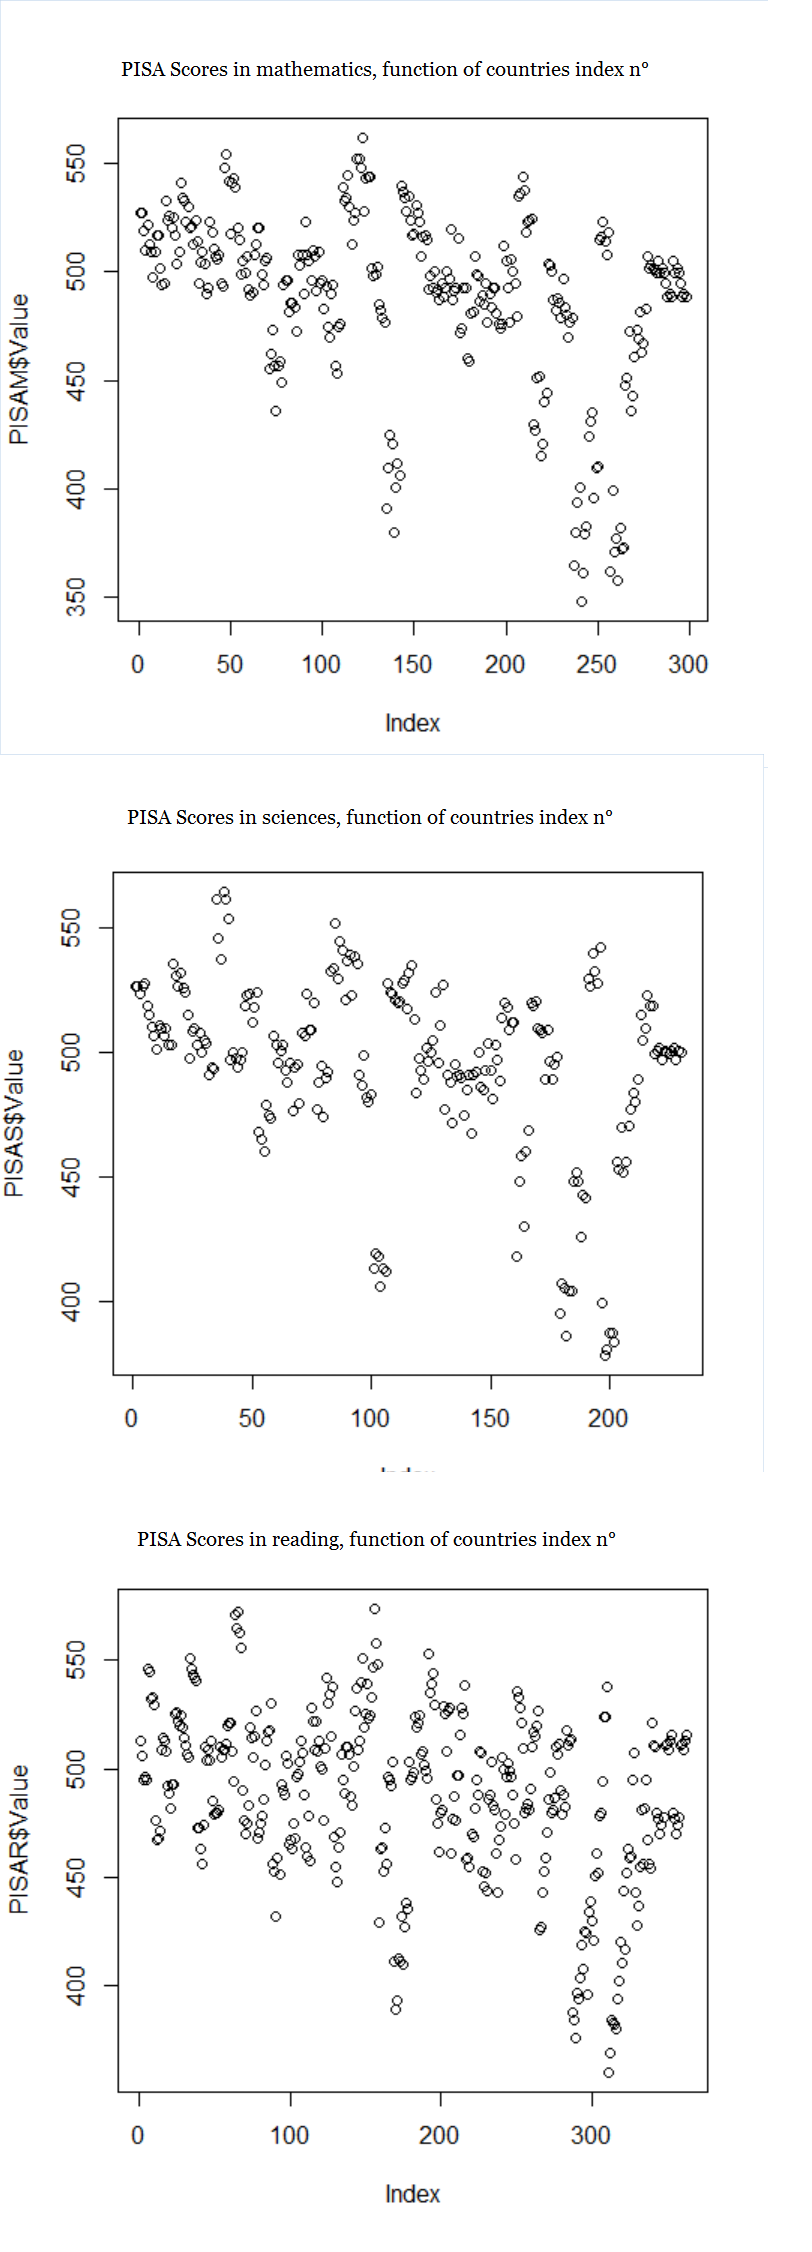
\includegraphics[scale=0.4]{img/IntraDependencePISA.png}
\end{figure}

Therefore the results in PISA in maths and in sciences will be treated as one set of results in what follows. Reading results will be treated independently.

\section{Methodology of analysis}

\subsection{Exemple of script used for analysis}

The following part details the generic script skeleton that the authors used to determine dependencies between academic factors and PISA results in mathematics and in reading.

Let us consider the exemple of the script assessingthe influence of the $\frac{N_{students}}{N_{teachers}}$ ratio on the results at PISA.
The first part is about loading the right R libraires for analysis:
\begin{lstlisting}
## LOADING LIBRARIES ##
library(MASS)
library(sqldf)
library(entropy)
setwd("D:/PISA_Results_Analysis/Data")
\end{lstlisting}

Then we load the CSV files that we will use in the script. Note that PISA results were processed only for girl students. This is justified by the fact that standard deviation is lower for girl students than it is for boys students.
\begin{lstlisting}
## LOADING AND FILTERING PISA MATHS DB ##
> PISAMFile <- "PISA_Maths.csv"
> PISAM <- read.csv(PISAMFile)
> colnames(PISAM) <- c("CTR", "INDICATOR", "SUBJECT", "MEASURE",
+ "FREQUENCY", "TIME", "Value", "Flag.Codes")
> PISAMFilt <- sqldf("select CTR, Value from PISAM where
+ SUBJECT=='GIRL' and TIME=='2012'")
> head(PISAMFilt)

## LOADING AND FILTERING PISA READING DB ##
> PISARFile <- "PISA_Reading.csv"
> PISAR <- read.csv(PISARFile)
> colnames(PISAR) <- c("CTR", "INDICATOR", "SUBJECT", "MEASURE",
+ "FREQUENCY", "TIME", "Value", "Flag.Codes")
> PISARFilt <- sqldf("select CTR, Value from PISAR where
+ SUBJECT=='GIRL' and TIME=='2012'")
> head(PISARFilt)

## LOADING CSV FILE ABOUT S/T RATIO ##

> STFile <- "Stud_Teach_Ratio.csv"
> ST <- read.csv(STFile)
> colnames(ST) <- c("CTR", "Country", "LVL", "Level of education", "SCT",
+ "Reference sector", "IND", "Indicator", "YEA", "Year", "UNT", "Unit",
+ "PWC", "PowerCode", "PER", "Reference Period", "Value", "FLG", "Flags")
\end{lstlisting}
Then a mere SQL request is enough to select only the interesting variables among those in the file.
\begin{lstlisting}
> STRatio <- sqldf("select CTR, Value from ST where IND=='PERS_RATIO_INST'
+ and SCT=='INST_T' and LVL=='L2_3'")
\end{lstlisting}
The constructed dataset is then merged with the PISA dataset so that its influence on the results at PISA can be studied.
\begin{lstlisting}
> STM <- merge(STRatio,PISAMFilt,by = "CTR")			# 37 entries
> STM <- na.omit(STM)							# 32 entries
> colnames(STM) <- c("CTR", "S/T ratio", "PISA Maths Score")

> STR <- merge(STRatio,PISASFilt,by = "CTR")			# 37 entries
> STR <- na.omit(STR)							# 32 entries
> colnames(STR) <- c("CTR", "S/T ratio", "PISA Reading Score")
\end{lstlisting}
The next step often is to discretize the distribution that we have. Let us remind the reader that we would like to test the dependence of the S/T ratio on results at PISA, both in mathematics and at reading. To assess dependence the exact Test of Fisher was used. A piece of justification would be that the datasets are too small for the $\Xi$-squared approximation to be true in this situation. Fisher tests are often used in situations with a small number of entries, which is the case here.
To do this the authors used the "entropy" library. One of the major drawbacks of this method is that the results of the Fisher tests depend on the binning, that is the level at which our datasets are discretized.
In this study two binning numbers were used for each academic factor studied. Each time the authors tried to take a number of bins as high as possible, to get a good discrete representation of the datasets.
\begin{lstlisting}
> Discrete_ST_M8 <- discretize2d(STM$"S/T ratio", STM$"PISA Maths Score",
+ numBins1=8, numBins2=8)
> Discrete_ST_M12 <- discretize2d(STM$"S/T ratio", STM$"PISA Maths Score",
+ numBins1=12, numBins2=12)
> Discrete_ST_R8 <- discretize2d(STS$"S/T ratio", STS$"PISA Sciences Score",
+ numBins1=8, numBins2=8)
> Discrete_ST_R12 <- discretize2d(STS$"S/T ratio", STS$"PISA Sciences Score",
+ numBins1=12, numBins2=12)

> STFisherM8 <- fisher.test(Discrete_ST_M8)
	# Fisher's Exact Test for Count Data
	# data:  Discrete_ST_M8
	# p-value = 0.09221
	# alternative hypothesis: two.sided
> STFisherS8 <- fisher.test(Discrete_ST_S8)
	# Fisher's Exact Test for Count Data
	# data:  Discrete_ST_R8
	# p-value = 0.1772
	# alternative hypothesis: two.sided
\end{lstlisting}
At last here is the plot of PISA results as a function of $\frac{N_{students}}{N_{teachers}}$
\begin{lstlisting}	
# Plot of PISAMaths = f(S/T) #
> plot(STM$"S/T ratio", STM$"PISA Maths Score")

# Plot of PISAReading = f(S/T) #
> plot(STR$"S/T ratio", STR$"PISA Reading Score")
\end{lstlisting}

\begin{figure}
	\centering
	\label{STRatio}
	\caption{Influence of the student/Teacher ratio on the results at PISA}
	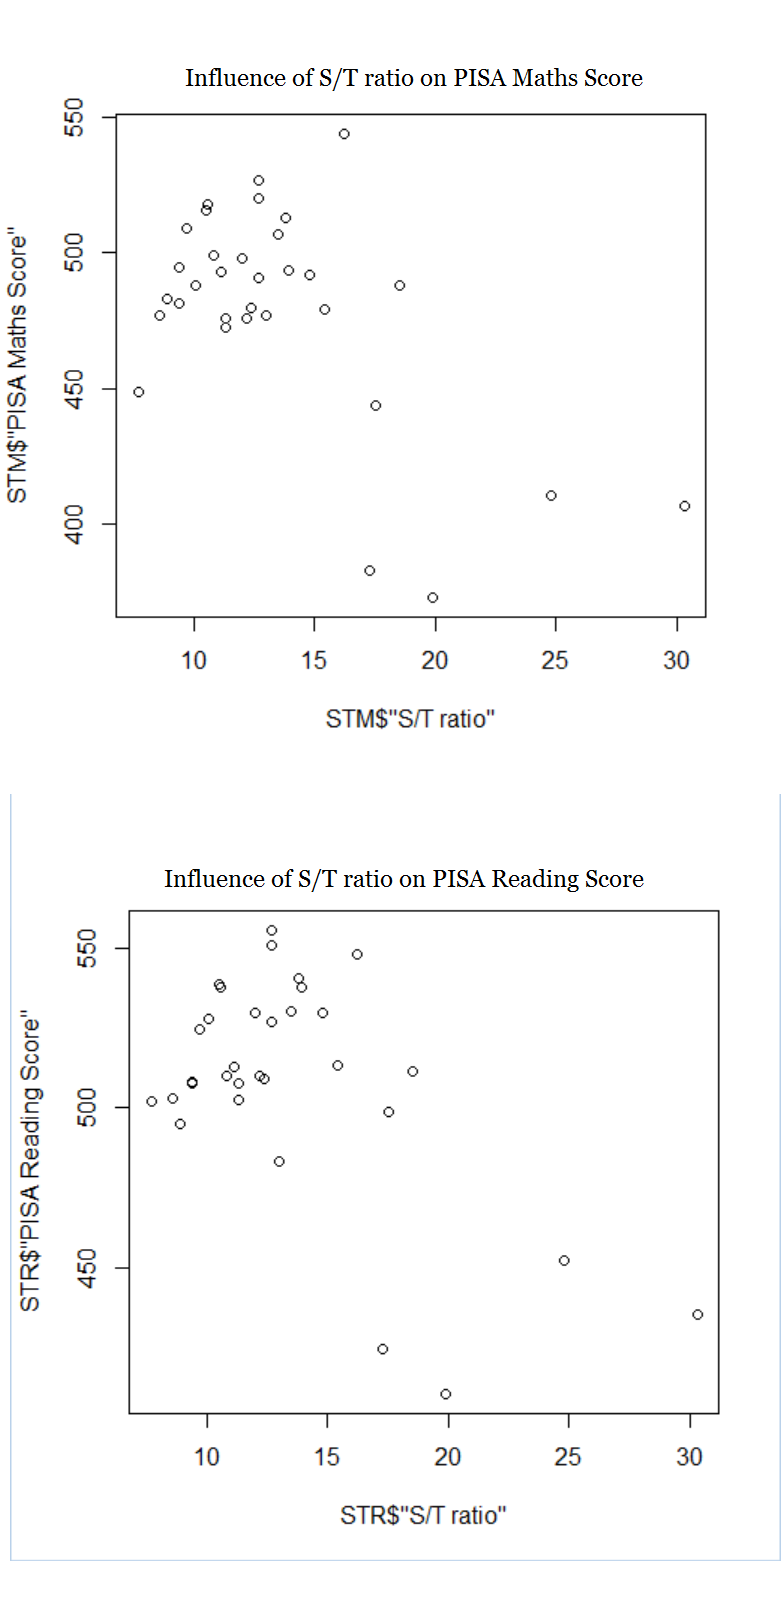
\includegraphics[scale=0.4]{img/STRatio.png}
\end{figure}

\subsection{Amount of available data}

The most limitating factor in this study is the small number of entries. As data emanates from different databases, some data are given for every year from 2000 to 2012, others only are available for 2012...
What the authors did when possible is that they've used data from several years in order to have more entries. As there only is PISA data for the years 2006, 2009 and 2012, this process is possible for a factor if there is data for at least two of those years for this same factor.
This was namely the case for the \textit{teaching hours} factor.

Of course one of the critics that can be addressed to the authors is that they treated data from 2006 the same way they treated data from 2012, despite knowing that they cannot know how trends have evolved between 2006 and 2012. As we only study a few factors, and as the results of this study points out, the factors that the authors studied do not completely represent the results at PISA, which means that there is a mechanism that the authors failed to find. By treating data from 2006 and 2012 the same way, the authors made the hypothesis that:
\begin{itemize}
	\item some countries give significantly different results three years apart
	\item there is no hidden or ignored variable that could influence the PISA results and significantly vary in three years
\end{itemize}

\subsection{Strategy of analysis}

The study is divided in two parts:
\begin{enumerate}
	\item The study of the dependence of each academic factor to PISA results, both in mathematics and in reading. As presented just before and because of the small number of entries in the data frames, the exact Fisher Test was used. Therefore the scripts for different academic factors are very similar, which is why only one of the scripts is presented in this paper.
	\item A principal component analysis that aims at explaining the results at PISA in mathematics and reading, in order to know what factor significantly influences the results relatively to one another
\end{enumerate}

\section{Results}

\subsection{Student / Teachers ratio}

No data was found for the years 2009 or 2006. Therefore there were only 32 entries available for this test, which were those of year 2012.
For a number of bins of 8, the results show that \textbf{the $\frac{N_{students}}{N_{teachers}}$ is correlated to the results in science at PISA for 5\% and 3\% uncertainty index} (Fisher test, p\_value = $2.672*10^{-2}$). As the results at PISA in mathematics and science are slightly different, it is not necessarily surprising to find that the $\frac{N_{students}}{N_{teachers}}$ is not correlated to the results in maths (the p\_value is quite low though, p\_value = $9.152*10^{-2}$).

No correlation between the previous ratio and the results at the reading test was found.

For a graphic representation of the results at PISA as a function of $\frac{N_{students}}{N_{teachers}}$, refer to \ref{STRatio}.

\subsection{Are PISA results representative of the tertiary diplomas rate? }

The previous analysis was led by presuming that results at PISA would reveal a tendency. The authors have decided to sum up the academic performance of a country not by its results at PISA tests, but by the rate of tertiary diplomas in this country. As a matter of fact, PISA tests are often criticised for not being able to judge the performance of education because of the strong cultural and contextual discrepancies in the collection of countries that take part to the tests.

This sections aims at asserting if the two variables - results at PISA in one of the fields, and the rate of people with a tertiary diploma (bachelor, master of PhD) - are linked whatsoever.

\begin{figure}
	\centering
	\label{3DRate}
	\caption{Tertiary diploma rate as a function of results at PISA. The reader will notice the trend that is represented here: overall better results at PISA lead to a greater rate of people with a tertiary diplomas}
	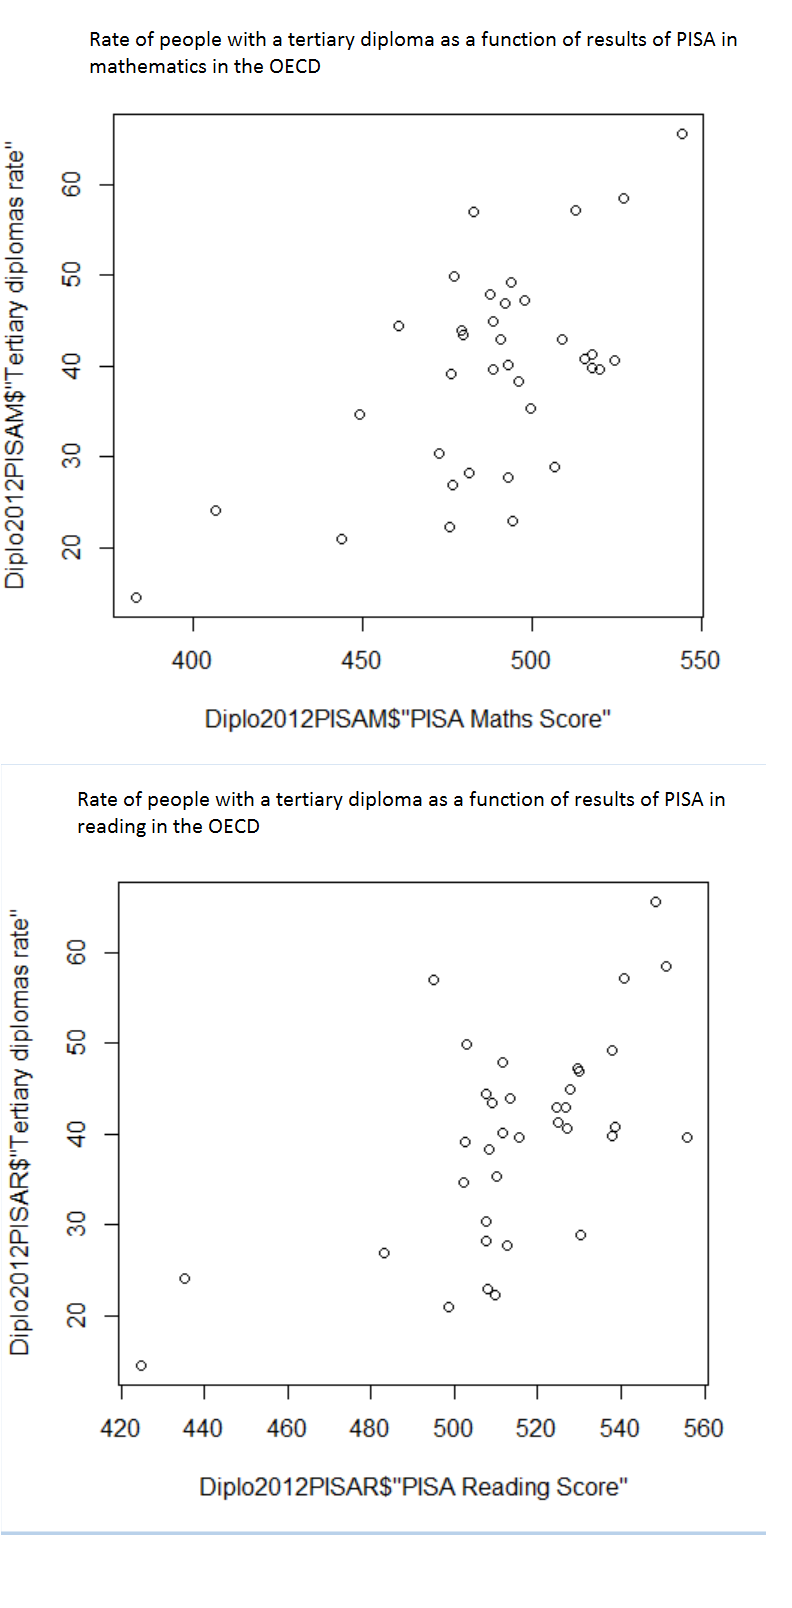
\includegraphics[scale=0.4]{img/3DRate.png}
\end{figure}

\section{Conclusion}

\section{Bibliography}

\end{document}